\documentclass[12pt, a4paper]{book}
\begin{document}

\chapter{BDT of depth 30}\label{apendix:BDT_depth_30}
Before conducting the final grid search for the final networks used on the results, we experimented with different hyperparameters to change. On one of grid searches we set the learning rate as $\eta=0.1$ 
as the trend showed this giving the best results with less overtraining, and $\lambda=10^{-5}$. This grid search had \verb|n_estimators| $\in[10, 100, 500, 1000]$ and depth $\in[3,4,5,6]$. 
The expected significance is shown in Figure \ref{fig:BDT_sig}. The testing and training AUC can be seen in Figure \ref{fig:BDT_GRID_AUC}.
\graphicspath{{../../Plots/XGBoost/FULL/GRIDSEARCH_n_est_10-1000}}
\begin{figure}[!ht]
   \centering
   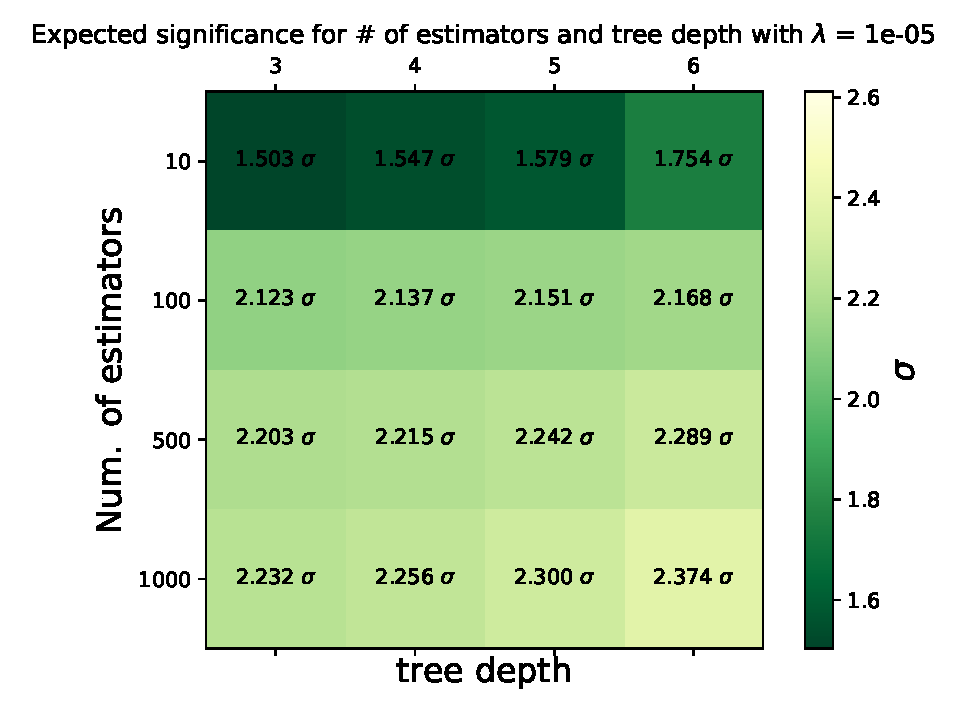
\includegraphics[width=0.6\textwidth]{Expected_significance.pdf}  
   \caption{Grid search expected significance when setting $\lambda=10^{-5}$ and $\eta=0.1$}\label{fig:BDT_sig}
\end{figure}
\begin{figure}[!ht]
\centering
\begin{subfigure}[b]{0.49\textwidth}
      \centering
      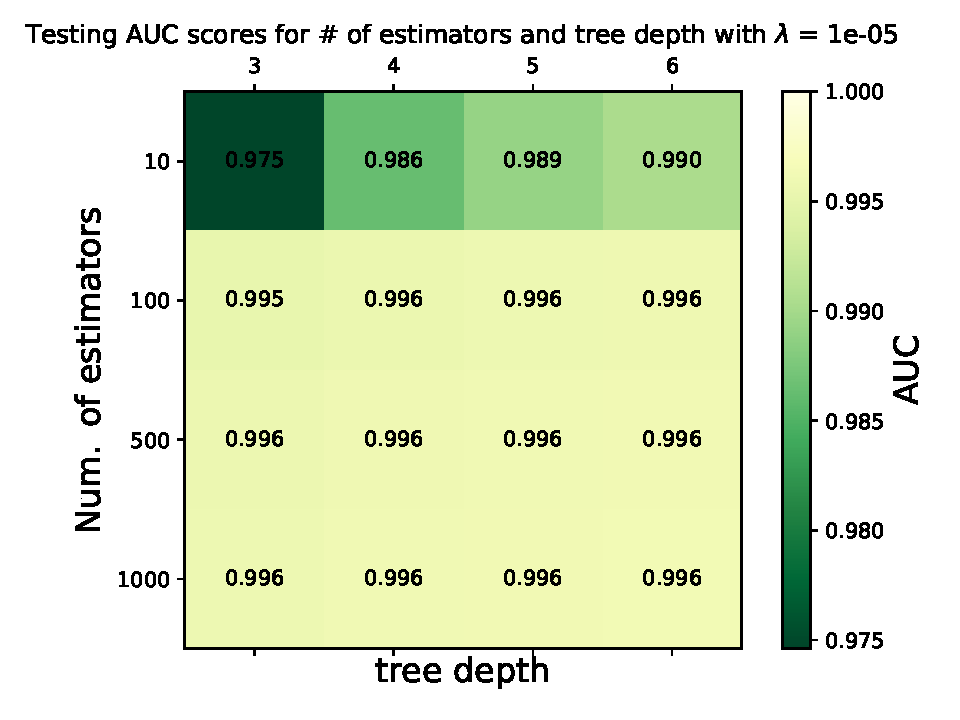
\includegraphics[width=1\textwidth]{Testing_AUC.pdf}
      \caption{Testing AUC}
   \end{subfigure}
   \hfill
   \begin{subfigure}[b]{0.49\textwidth}
      \centering
      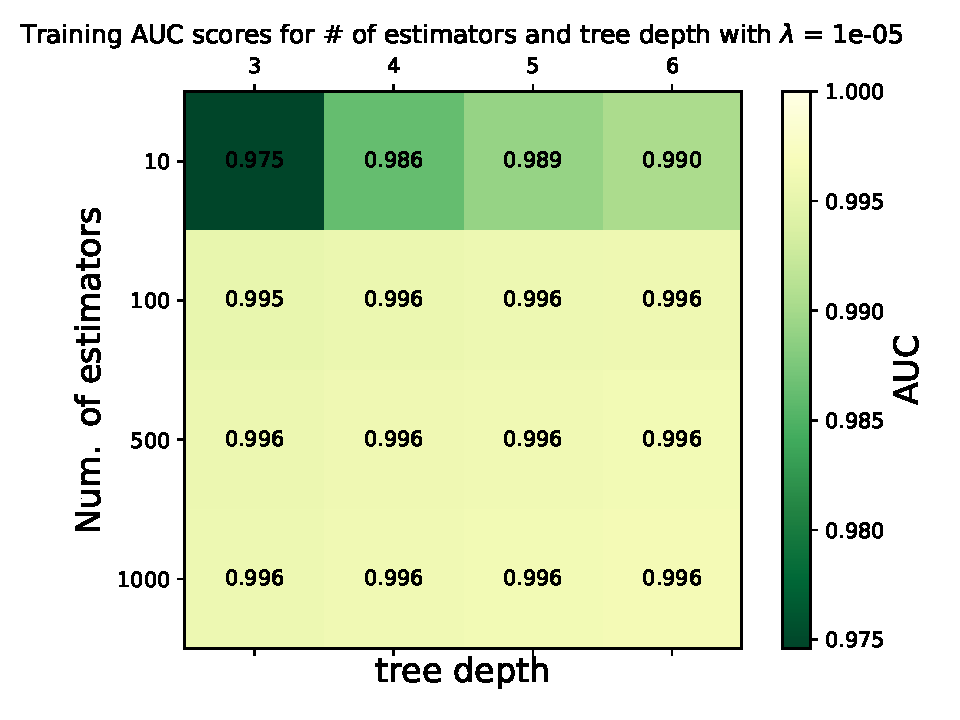
\includegraphics[width=1\textwidth]{Training_AUC.pdf}
      \caption{Training AUC}
   \end{subfigure}
   \caption[Grid search result for BDT]{Grid search AUC when setting $\lambda=10^{-5}$ and $\eta=0.1$}\label{fig:BDT_GRID_AUC}
\end{figure}
\\The best networks (depth of 6 and 1000 estimators) feature importance plots is shown in Figure \ref{fig:BDT_feat}.\\
\graphicspath{{../../Plots/XGBoost/FULL/GRIDSEARCH_n_est_10-1000/DH_HDS_mZp_130/feature_importance/}}
\begin{figure}[!ht]
	\centering
   \begin{subfigure}[b]{0.8\textwidth}
      \centering
      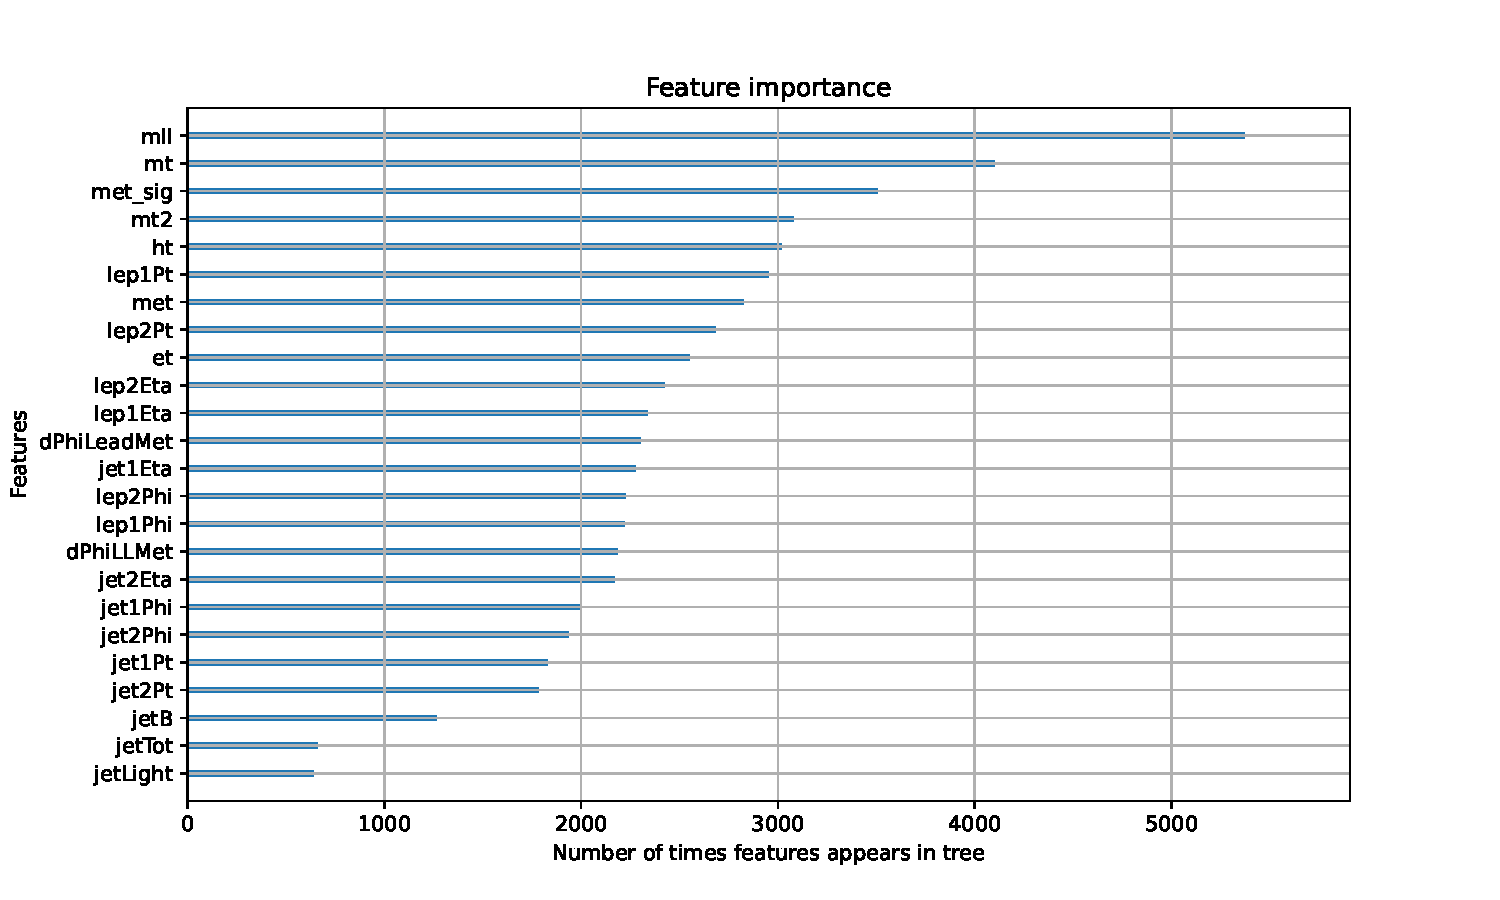
\includegraphics[width=1\textwidth]{weight.pdf}
      \caption{Using "weight" metric}
   \end{subfigure}
   \hfill
   \begin{subfigure}[b]{0.8\textwidth}
      \centering
      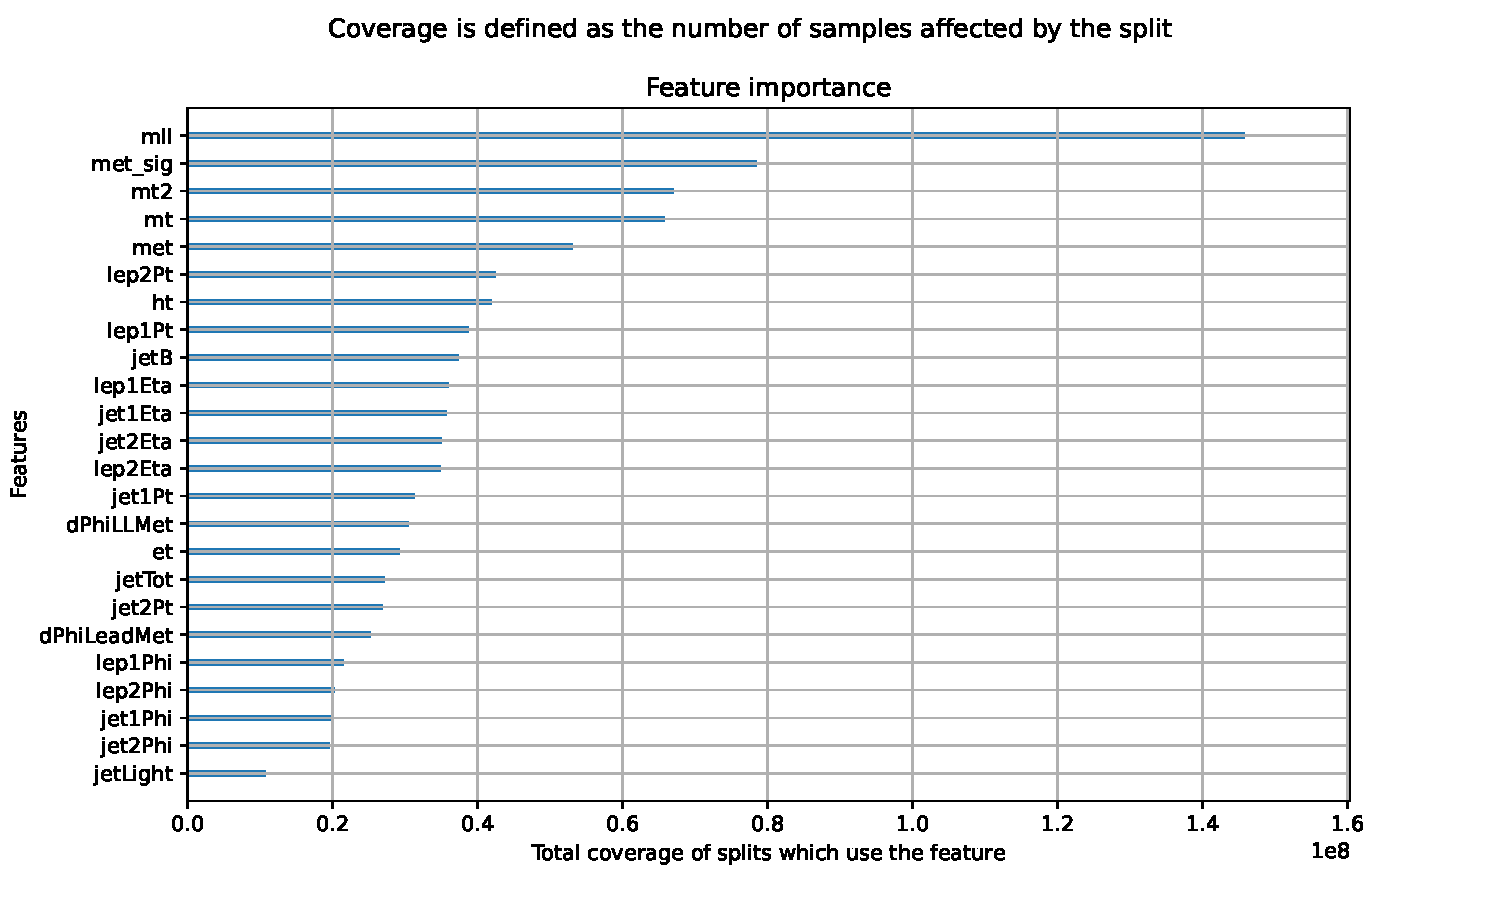
\includegraphics[width=1\textwidth]{total_cover.pdf}
      \caption{Using "coverage" metric}
   \end{subfigure}
   \caption[Feature importance plots of BDT]{Feature importance of depth 6 network trained on FULL Z' DM data set when testing it on DH HDS $m_{Z'}=130$ GeV model.}\label{fig:BDT_feat}
\end{figure}
\\However, as we can on Figure \ref{fig:BDT_sig} the expected significance does not seem to converge. Because of this, and out of curiosity we decided to keep training the networks with a greater depth. 
The results can be shown in Figure \ref{fig:BDT_deep_sig}. \\
\graphicspath{{../../Plots/XGBoost/FULL/GRIDSEARCH_3-6}}
\begin{figure}[!ht]
	\centering
	\begin{subfigure}[b]{0.49\textwidth}
      \centering
      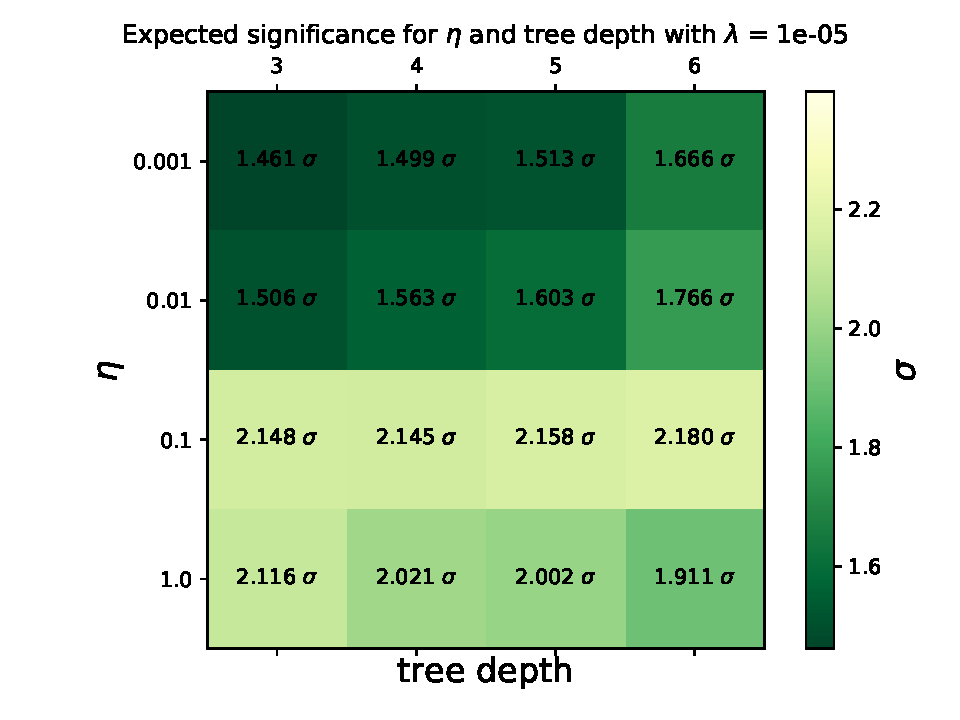
\includegraphics[width=1\textwidth]{Expected_significance.pdf}
   \end{subfigure}
   \hfill\graphicspath{{../../Plots/XGBoost/FULL/GRIDSEARCH_24-30}}
   \begin{subfigure}[b]{0.49\textwidth}
      \centering
      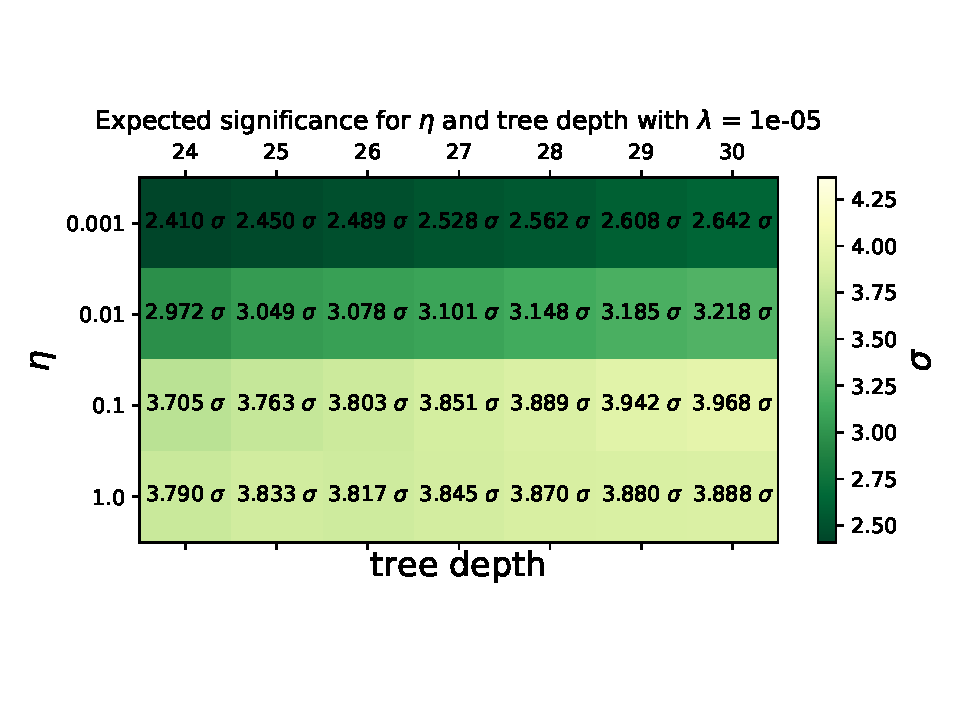
\includegraphics[width=1\textwidth]{Expected_significance.pdf}
   \end{subfigure}
   \caption{Grid search expected significance going to a depth of up to 30}\label{fig:BDT_deep_sig}
\end{figure}
\\In the Figure we see that the networks expected significance does not seem to converge, and rather just keeps getting greater and greater. 
This is however highly radical as the convention is to normally not have a depth greater than 7, which already is radical. The reason for not having deep BDTs being that the network is highly likely to overtrain and give wrong predictions. 
However, this was not the case for us as seen for example in Figure \ref{fig:DBDT_GRID_AUC}.\\
\graphicspath{{../../Plots/XGBoost/FULL/GRIDSEARCH_24-30}}
\begin{figure}[!ht]
\centering
\begin{subfigure}[b]{0.49\textwidth}
      \centering
      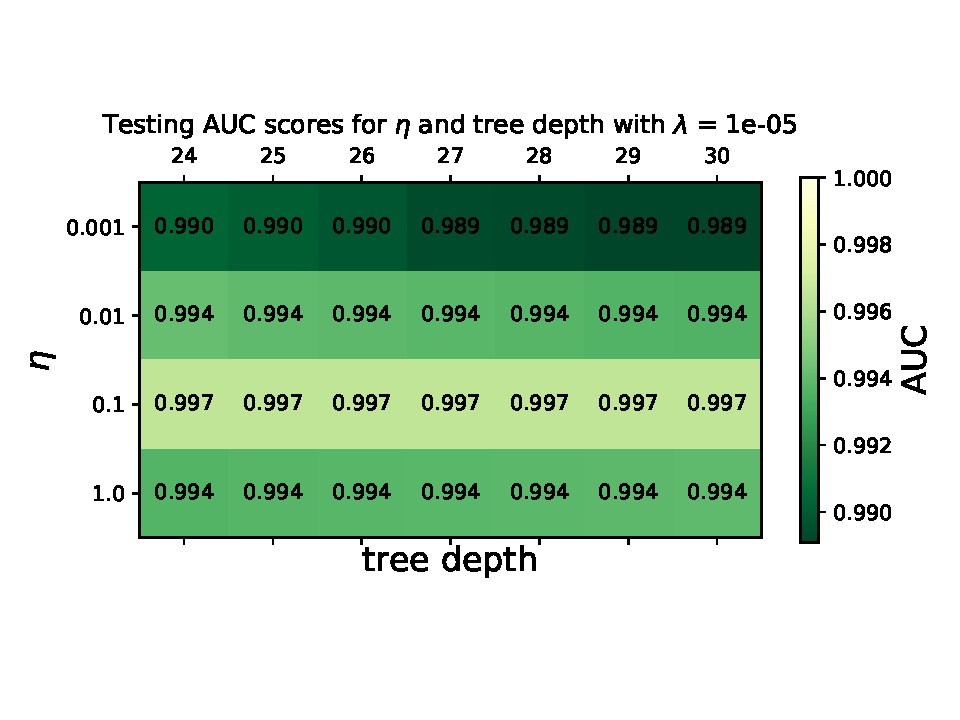
\includegraphics[width=1\textwidth]{Testing_AUC.pdf}
      \caption{Testing AUC}
   \end{subfigure}
   \hfill
   \begin{subfigure}[b]{0.49\textwidth}
      \centering
      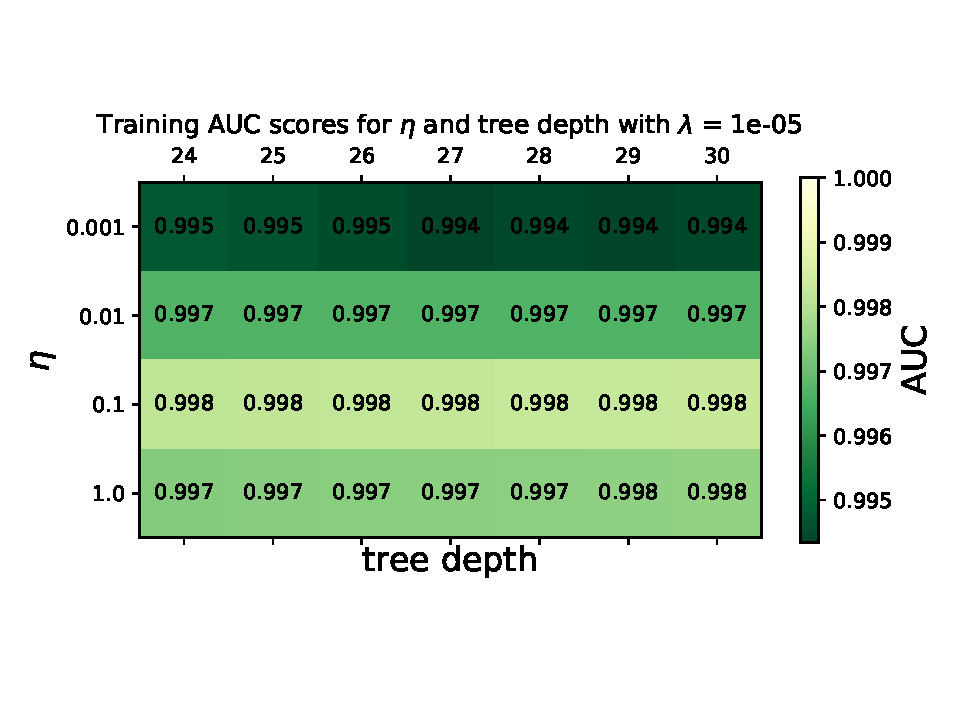
\includegraphics[width=1\textwidth]{Training_AUC.pdf}
      \caption{Training AUC}
   \end{subfigure}
   \caption{Grid search AUC going to a depth of up to 30}\label{fig:DBDT_GRID_AUC}
\end{figure}
\\ I understand however that this is controversial since we are splitting a data set, that is at best of size $2^{27}$, 30 times. That means that after a depth of 27 there is exactly one event pr branch.
So how does a depth of 30 make sense? To help with this we could use a feature in XGBoost to see which features are most important when evaluating a signal. 
When testing the network trained on the FULL Z' DM data set on a DH HDS $m_{Z'}=130$ GeV model we get the features shown in Figure \ref{fig:DBDT_feat} as most important. 
\graphicspath{{../../Plots/XGBoost/FULL/DH_HDS_mZp_130/feature_importance}}
\begin{figure}[!ht]
	\centering
   \begin{subfigure}[b]{0.8\textwidth}
      \centering
      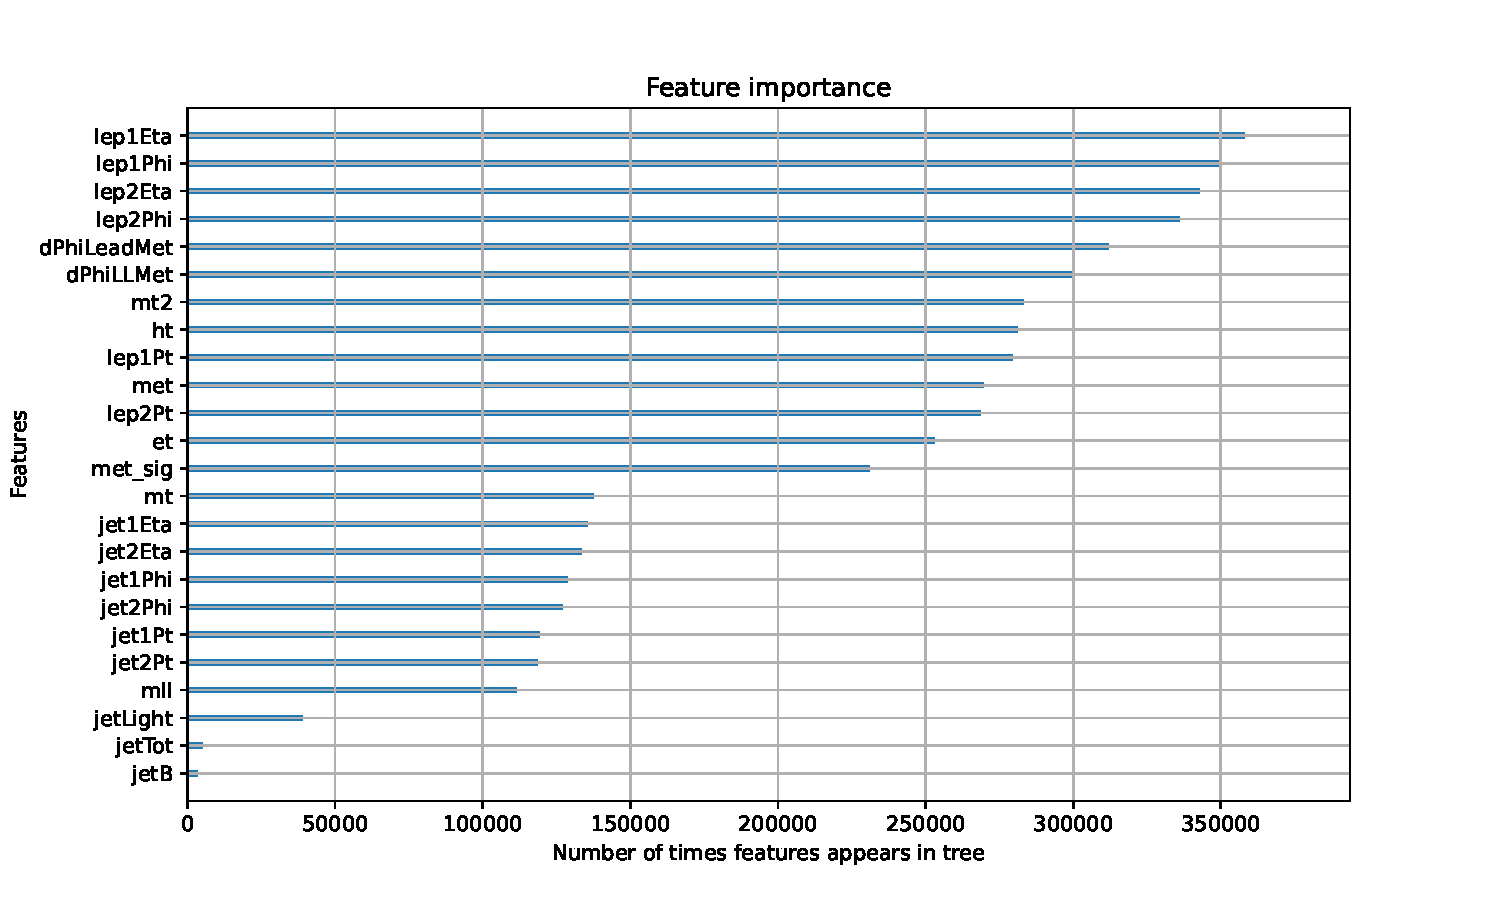
\includegraphics[width=1\textwidth]{weight.pdf}
      \caption{Using "weight" metric}
   \end{subfigure}
   \hfill
   \begin{subfigure}[b]{0.8\textwidth}
      \centering
      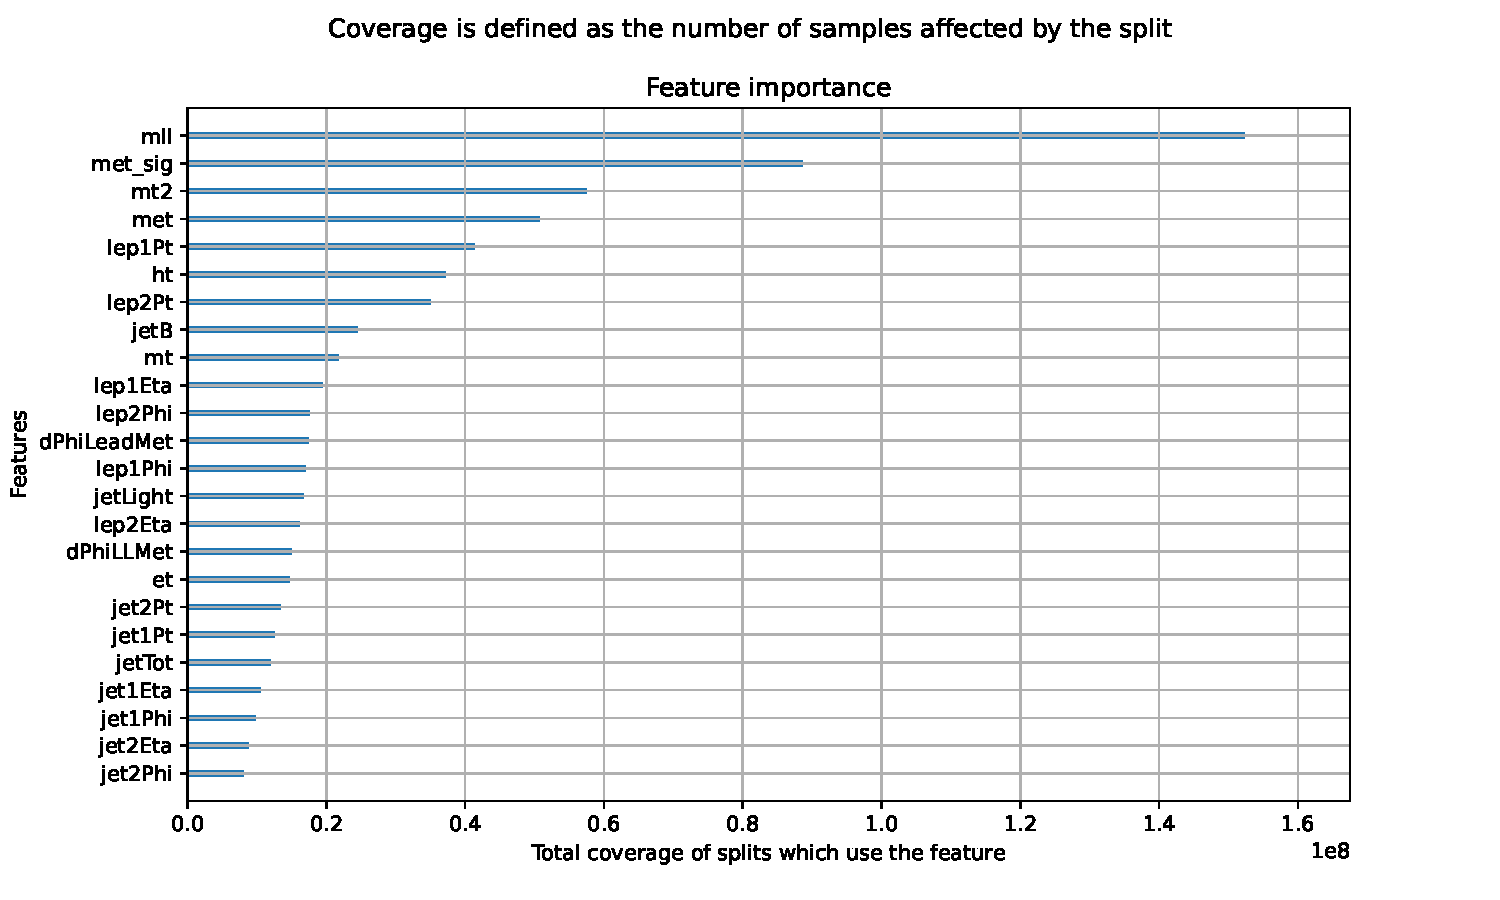
\includegraphics[width=1\textwidth]{total_cover.pdf}
      \caption{Using "coverage" metric}
   \end{subfigure}
   \caption{Feature importance of depth 30 network trained on FULL Z' DM data set when testing it on DH HDS $m_{Z'}=130$ GeV model.}\label{fig:DBDT_feat}
\end{figure}
\newpage\noindent As we can see these features vary a lot depending on which metric we use to evaluate the importance. 
When using the "coverage" metric, which as stated is defined as the number of samples affected by the split, we get the features we physically expect to be important when trying to single out a DM model.
And this metric is arguably the one we need to use to define what features are important. Since the more samples a feature split, the more powerful it is to separate signal from background.\\
\\We can see however that when we use "weight" as a metric, which is the XGBoost standard metric, we get completely unexpected features that we physically don't expect to be important when trying to single out a DM model.
But as described by the metric, the "weight" is the number of times a feature appears in a tree. Which might explain that the reason the pseudorapidity and $\phi$ range so high on this list, 
is simply because the tree is struggling to find a pattern here and is trying extra hard to single out DM from SM. \\
\\To showcase the difference in signal recognition between the monstrous 30 depth BDT to the more sensible 6 depth BDT, I again tested the networks on the good old DH HDS $m_{Z'}=130$ GeV model.
The results as well as their expected significance can be seen below.
\begin{figure}[!ht]
	\centering
   \graphicspath{{../../Plots/XGBoost/FULL/GRIDSEARCH_n_est_10-1000/DH_HDS_mZp_130/}}
	\begin{subfigure}[b]{0.49\textwidth}
        \centering
        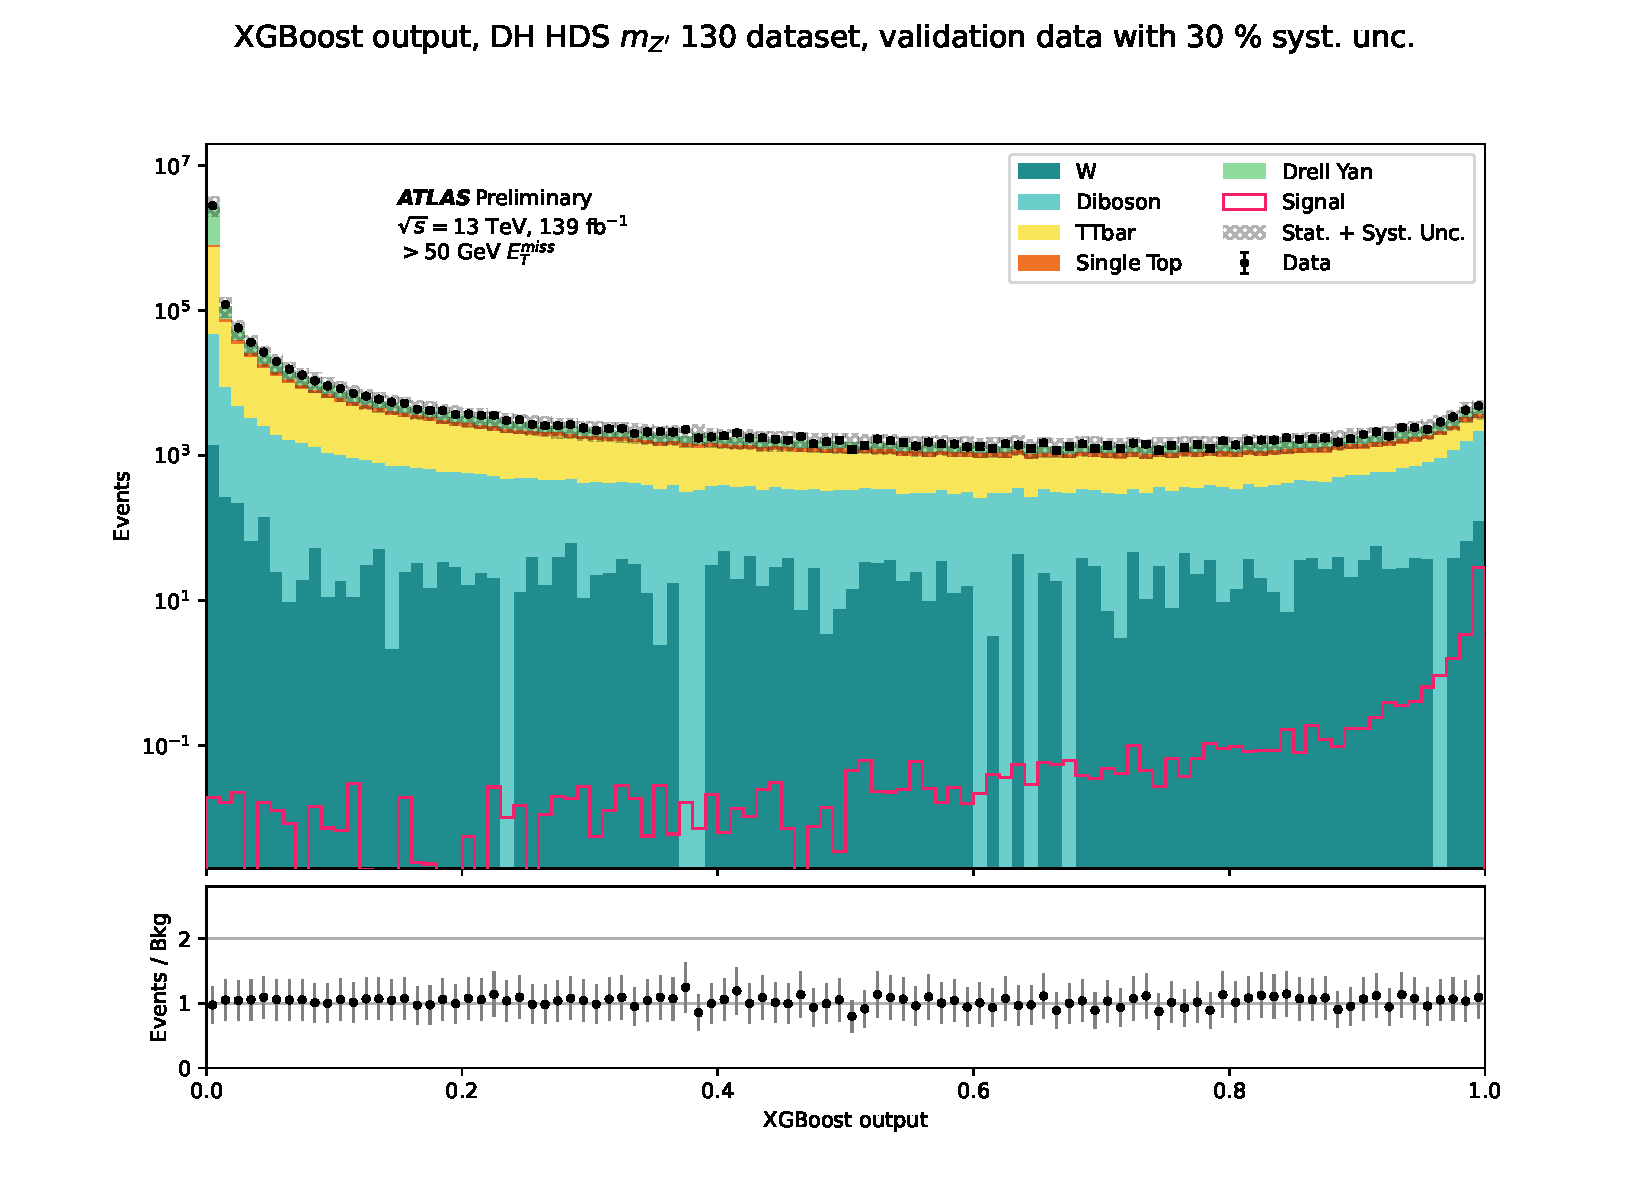
\includegraphics[width=1\textwidth]{VAL.pdf}
        \caption{Depth of 6}
     \end{subfigure}
     \hfill\graphicspath{{../../Plots/XGBoost/FULL/DH_HDS_mZp_130/}}
     \begin{subfigure}[b]{0.49\textwidth}
        \centering
        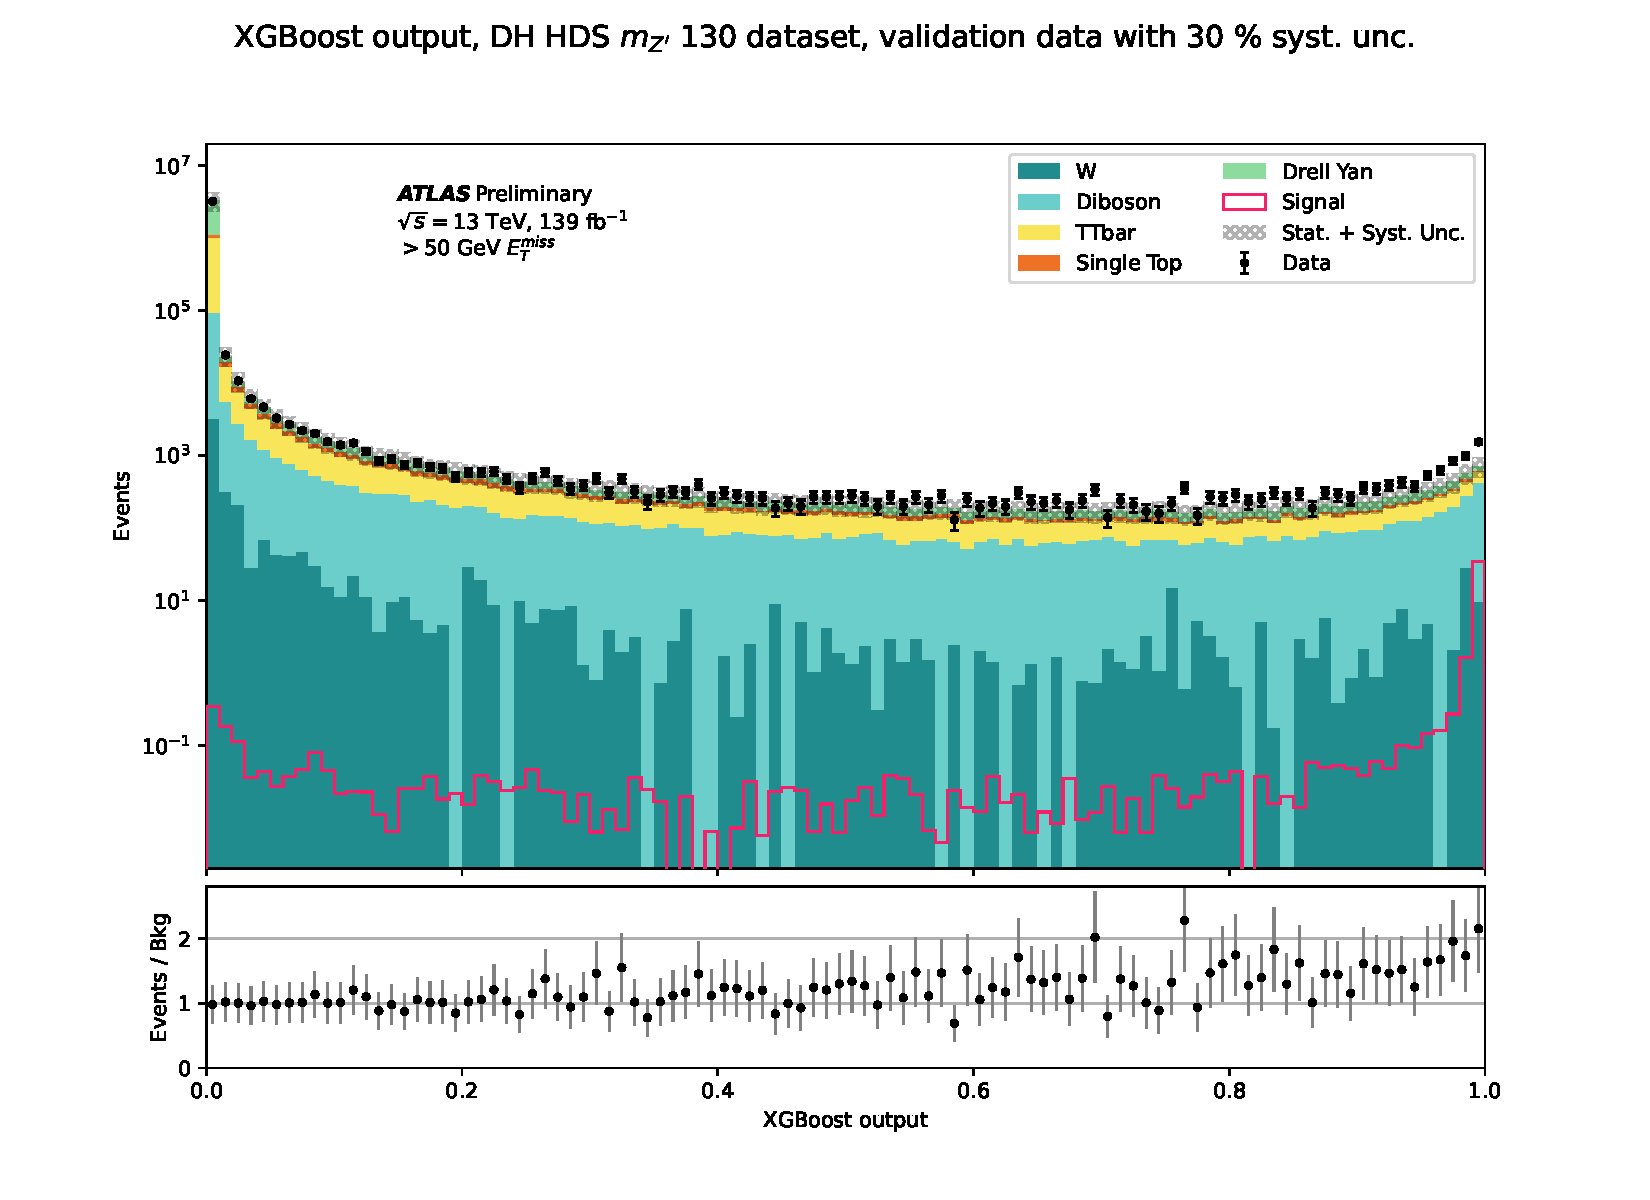
\includegraphics[width=1\textwidth]{VAL.pdf}
        \caption{Depth of 30}
     \end{subfigure}
   \hfill\graphicspath{{../../Plots/XGBoost/FULL/GRIDSEARCH_n_est_10-1000/DH_HDS_mZp_130/}}
   \begin{subfigure}[b]{0.49\textwidth}
      \centering
      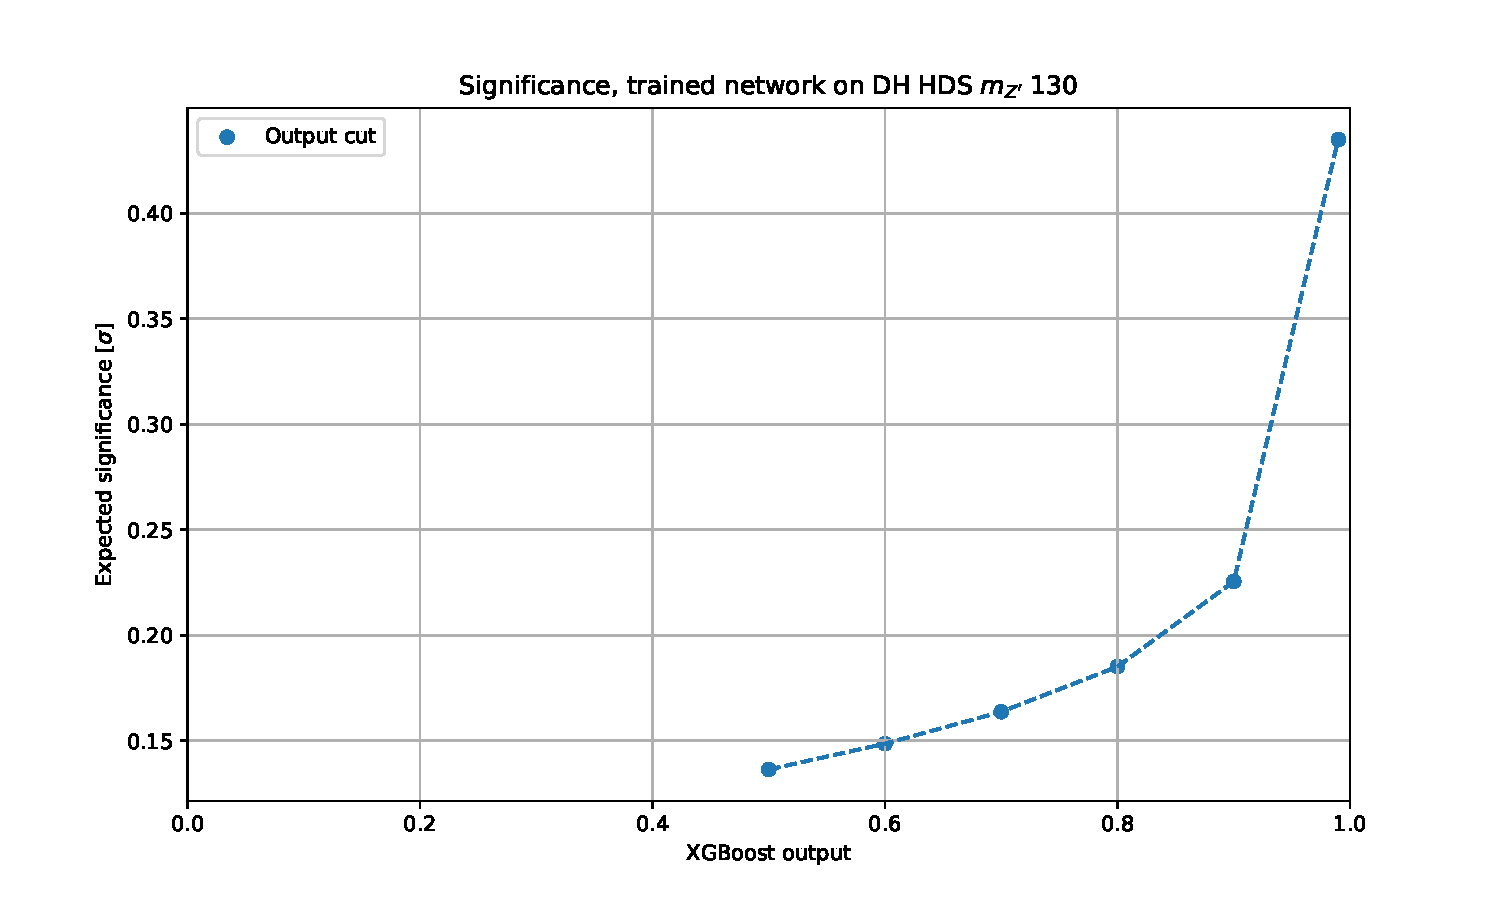
\includegraphics[width=1\textwidth]{EXP_SIG.pdf}
      \caption{The expected significance of a)}
   \end{subfigure}
   \hfill\graphicspath{{../../Plots/XGBoost/FULL/DH_HDS_mZp_130/}}
   \begin{subfigure}[b]{0.49\textwidth}
      \centering
      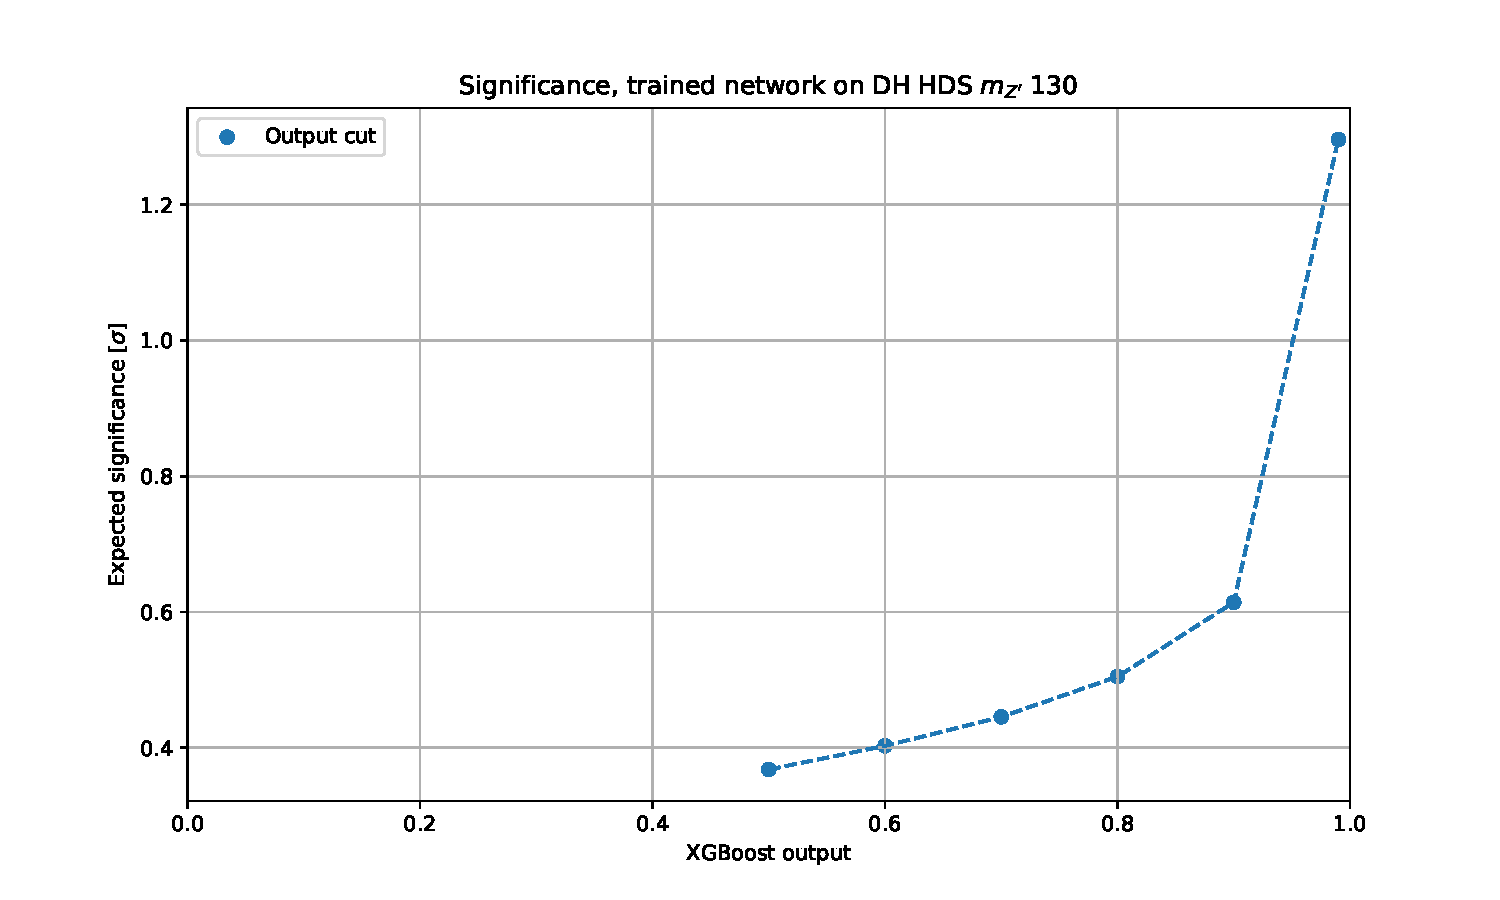
\includegraphics[width=1\textwidth]{EXP_SIG.pdf}
      \caption{The expected significance of b)}
   \end{subfigure}
   \caption{Comparison of the network performance when having a depth of 6 and 30. Figure a) and b) show the validation data of both cases, c) and d) show the expected significance of the validation plots when making a cut on the output. }
\end{figure}
\\The difference is extreme, when looking at the monster of depth 30 we can get an expected significance of 1.2 $\sigma$ (without uncertainties) on our model of max 15 events, only having made a cut of 50 GeV on the missing transverse energy.
We can however see that the data and background do not agree to the same degree of the network with depth 6. Using purely statistical uncertainty and assuming a systematic uncertainty of 30\%, we see that a few data points do not agree with the MC background.
These data points are points the network classified as signal, so if we completely trusted the network this would be a hint of new physics! 
However, this is the last thing we should assume, and rather take this as a hint that the network is doing something fishy.\\
\\If I had access to XGBoost with built GPU support, I would increase the number of estimators even more to check if this increases the significance while still having a depth of maximum 6.
However, as of now this is not possible. As the weighting method explained in the previous section was not included here, we will drop going to a tree depth of 30, and have a maximum of 6.


\end{document}